\section{Theorie}
\label{sec:Theorie}
\subsection{Grundlagen der magnetischen Kernresonanz}
Die meisten Atomkerne besitzen neben Kernladung und Masse, auch einen Eigendrehimpuls, welcher als Spin $I$ bezeichnet wird.
Der Spin und das magnetische Dipolmoment des Atomkerns sind wie folgt miteinander verkn\"{u}pft:
\begin{align*}
	\overrightarrow{\mu} = \hbar \gamma \overrightarrow{I}
\end{align*}
hierbei ist $\gamma$ das gyromagnetische Verh\"{a}ltnis, welches element- und isotopenspezifisch ist.

In einem \"{a}u{\ss}eren Magnetfeld $\overrightarrow{B_0}$ richten sich die magnetischen Dipolmomente der Atomkern aus.
Klassisch betrachtet ist die Energie dann abh\"{a}ngig vom Relativwinkel zwischen $\overrightarrow{\mu}$ und $\overrightarrow{B_0}$.
In der quantenmechanischen Betrachtung sind jedoch nur bestimmte Winkel zugelasssen.
Erlaubt sind die Winkeleinstellungen, welche folgende Bedingung erf\"{u}llen:
\begin{align}
	E &= -m \hbar \gamma_I B_0  \\
	\text{mit:} \, \, \,  m &= +I, +(I-1), ..., -(I-1), -I \nonumber
\end{align}
In einem \"{a}u{\ss}eren Magnetfeld befinden sich die Atomkerne somit auf verschiedenen Energieniveaus.
Atome mit einem Kernspin von $I=\frac{1}{2}$ sind die wichtigsten Kerne für die NMR-Spektroskopie.
%- "Zeeman-Effekt"
\begin{figure}[hbtp]
	\centering
	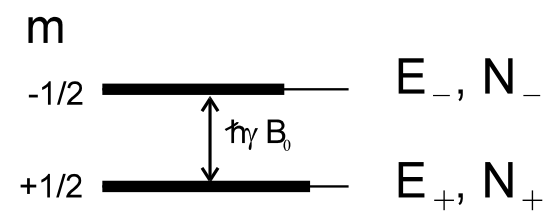
\includegraphics[width=0.5\textwidth]{Plots/energieniveaus.png}
	\caption{Aufspaltung der Energieniveaus f\"{u}r eine Atom mit Kernspin $\frac{1}{2}$.}
	\label{Energieniveaus}
\end{figure}
In Abbildung (\ref{Energieniveaus}) Aufspaltung der Energieniveaus f\"{u}r solche Atmoe zu sehen, mit der \"{U}bergangsenergie $\Delta E = \hbar \gamma B_0$.
Durch die unterschiedlichen Besetzungszahlen der einzelnen Niveaus kommt es zur  makroskopische Magnetisierung der Probe, dem Kernmagnetismus.
%- thermodynamischen Gleichgewicht Boltzmann-Verteilung
%- Kernmoment klein -> Ausrichtung durch externes Magnetfeld, Ausrichtung ist unab\"{a}ngig von der Orientierung der Molek\"{u}le
Zus\"{a}tzlich zu der Ausrichtung kommt auf Grund des Drehimpulses eine Pr\"{a}zessionsbewegung um $\overrightarrow{B_0}$ dazu.
Diese Pr\"{a}zessionsbewegung ist senkrecht zum externen Magnetfeld, womit der Winkel zwischen $\overrightarrow{\mu}$ und $\overrightarrow{B_0}$ zeitlich konstant ist.
- Lamorfrequenz: $\omega_0 = \gamma B_0$ hier: $\omega = 2\pi \cdot 90 \text{\, MHz}$
- wir betrachten die Summe aller Kernmomente: $M = \sum_i \mu_i$
- im Gleichgewicht ahebn alle die gleiche z-Komponente: $M = (0,0,M_z)$
- Gesamtmagnetisierung: $\frac{\vartheta M}{\vartheta t} = \gamma M_x B_0$
- $M und B_0$ sind parallel zueinander und damit zeitlich konstant
(- M kann auch pr\"{a}zidieren)

\paragraph{Rotierendes Koordinatensystem}
Da im folgenden senkrecht zu dem konstanten Magnet\-feld ein zeitliches Hochfrequenzfeld (HF-Feld) $B_1(t)$ hinzugeschaltet wird, wird hier nun zun\"{a}chst das rotierende Koordinatensystem als Konzept eingef\"{u}hrt.
In solch einem rotierenden Koordinatensystem ergeben sich $B_0$ und $B_1(t)$ zusammen zu einem effektiven Magnetfeld $B_{eff}$.
Dreht sich die Z-Achse beispielsweise mit der Frequenz $\Omega$, siehe Abbildung (\ref{rotK1}), um sich selbst, so gilt f\"{u}r die Gesamtmagnetisierung:
\begin{align*}
	\frac{dM}{dt} = \gamma M \times B - \Omega \times M = \gamma M \times \left(B - \frac{\Omega}{\gamma} \right)
\end{align*}
damit folgt f\"{u}r das effektive Magnetfeld:
\begin{align*}
	\frac{dM}{dt} = \gamma M \times B_{eff} \, \Rightarrow \, B_{eff} = B - \frac{\Omega}{\gamma}
\end{align*}
Somit wirkt das fiktive Feld $- \frac{\Omega}{\gamma}$ dem \"{a}u{\ss}eren Magnetfeld entgegen.
Das Hochfrequenzfeld wir mit einer Spule erzeugt und ist im Labor gegeben durch:
\begin{align*}
	B_1(t) = B_x cos(\Omega t)
\end{align*}
Im rotierenden Koordinatensystem wird diese HF-Feld in eine linke $B_{1,\text{links}}$ und eine rechte $B_{1,\text{rechts}}$ Komponente aufgeteilt, siehe Abbildung (\ref{rotK2}).
\begin{figure}[hbtp]
\caption{Rotierendes Koordinatensystem.}
\centering
	\begin{subfigure}[t]{0.4\textwidth}
	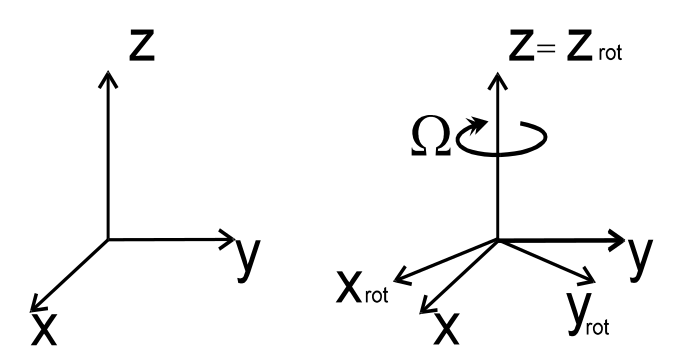
\includegraphics[width=\textwidth]{Plots/rotKoordinatensystem.png} 
	\subcaption{Die z-Achse rotiert mit Frequenz $\Omega$.}
	\label{rotK1}
	\end{subfigure}
	~
	~
	\begin{subfigure}[t]{0.4\textwidth}
	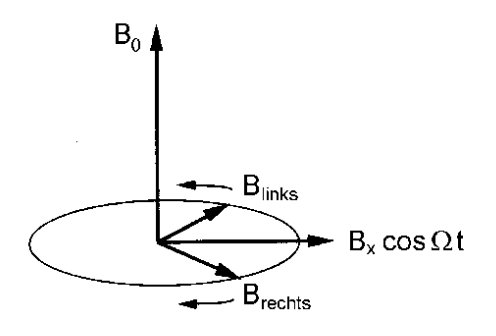
\includegraphics[width=0.8\textwidth]{Plots/B1Felder.png}
	\subcaption{Zeitabh\"{a}ngiges $B_1$-Feld wird in zwei Komponenten aufgeteilt, welche gegenl\"{a}ufig sind.}
	\label{rotK2}
	\end{subfigure}
\label{rotKoordi}
\end{figure}
Beide Komponenten rotieren mit einer Frequenz von $|\Omega|$ und einer Amplitude von $\frac{B_x}{2}$.
Nun kann die Komponente, die sich mit dem Koordinatensystem rotiert, als station\"{a}r betrachtet werden.
Im Gegenschluss rotiert dann die andere Komponente mit $-2\Omega$ und ist im Allgemeinen vernachl\"{a}ssigbar.

\paragraph{Die Auswirkungen von Hochfrequenzpulsen}
Um mit dem Hochfrequenzfeld, welches mit einer Spule erzeugt wird, einen Hochfrequenzpuls (HF-Puls) zu erzeugen, wird aus dem kontinuierlichen Feld der Spule ein Puls mit bestimmter L\"{a}nge herausgeschnitten, siehe Abbildung (\ref{HFPuls}).
\begin{figure}[hbtp]
	\centering
	\vspace{-10pt}
	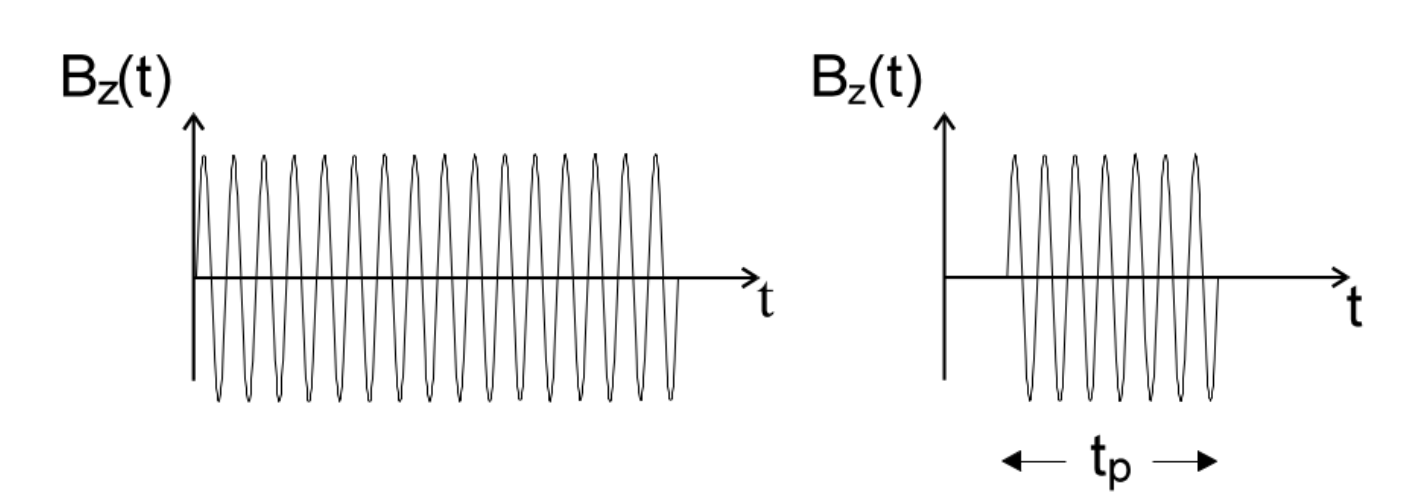
\includegraphics[width=0.55\textwidth]{Plots/HFPuls.png} 
	\label{HFpuls}
	\caption{Erzeugung eines HF-Pulses mit L\"{a}nge $t_p$.}
\end{figure}
Solch ein HF-Puls wei{\ss}t genau die L\"{a}nge $t_p$ auf, dass sich die Magnetisierung um $90^{\circ}$ dreht und sich eine Quermagnetisierung einstellt.
Daher wir der HF-Puls h\"{a}ufig auch als $90^{\circ}$-Puls oder $\frac{\pi}{2}$-Puls bezeichnet.
%- beliebigen Winkel $\alpha$ einstellen: $\omega_1 = \frac{\alpha}{t_p} \Rightarrow t_p = \frac{2 \alpha}{\gamma B_x}$
Nachdem ein $90^{\circ}$-Puls eingeschaltet wurde, pr\"{a}zediert die Magnetisierung $M$ um $\overrightarrow{B_0}$.
Diese Pr\"{a}zessionsbewegung der magnetischen Momente induziert dann eine Spannung in der Spule, in der die Probe sich befindet.
Es wird ein Kerninduktionssignal erzeugt.
Gemessen wird der Momentanwert 
\begin{wrapfigure}{r}{0.5\textwidth}
	\vspace{-10pt}
	\centering
	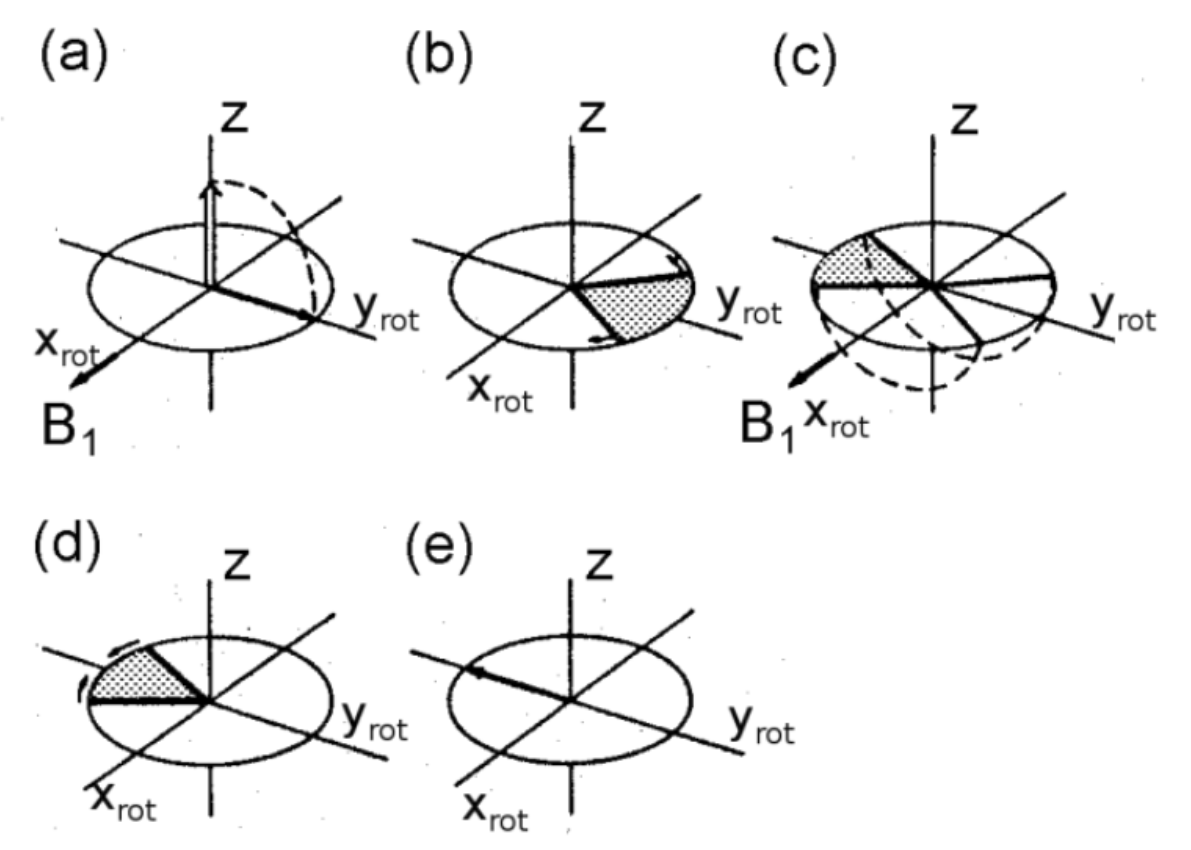
\includegraphics[width=0.45\textwidth]{Plots/hahnEcho.png} 
	\caption{Erzeugung eines Hahn-Echos durch die einen $90^{\circ}$-Puls (a) gefolgt von einem $180^{\circ}$-Puls (c).}
	\label{HahnEcho}
\end{wrapfigure}
der L\"{a}ngsmagnetisierung.
Die durch den $90^{\circ}$-Puls erzeugte Quermagnetisierung wird mit der Zeit kleiner, da die effektive Quermagnetisierung anf\"{a}ngt zu dephasieren, siehe Abbildung (\ref{HahnEcho}b).
Durch einen danach eingeschalteten $180^{\circ}$-Puls kommt es zur Rephasierung der Dipol{\-}mo{\-}men{\-}te (Abbildung (\ref{HahnEcho}d)).
Das Zusam{\-}men{\-}tref{\-}fen der Signalpunkte (Abbildung (\ref{HahnEcho}e)) wird als Hahn-Echo bezeichnet und kann gemessen werden.
Zu beachten ist, das die Magnetisierung im Hahn-Echo nicht der Magnetisierung nach dem $90^{\circ}$-Puls entspricht.
%- rotatorische und translatorische Molek\"{u}lbewegung -> Zerfall der Magnetisierung

\subsection{Relaxationen}
Die Magnetisierung $M(t)$ welche nach einen HF-Puls in der Probe vorliegt strebt wieder den Gleichgewichtswert $M_{eq}$ an.
Die Relaxation der Magnetisierung beruht auf der Wechselwirkung zwischen den Spins und deren Umgebung und wird in zwei Komponenten geteilt.
Zum Einen die longitudinale Relaxation entlang der z-Achse
\begin{align}
	\frac{d M_z(t)}{d t} = - \frac{M_z(t) - M_{eq}}{T_1} 
	\label{eq:bloch1}
\end{align}
und zum Anderen die transversale Relaxation in der x,y-Ebene
\begin{align}
	\frac{d M_{x,y}(t)}{d t} = - \frac{M_{x,y}(t)}{T_2}. 
	\label{eq:bloch2}
\end{align}
Diese beiden Gleichungen \eqref{eq:bloch1} und \eqref{eq:bloch2} sind als die Bloch-Gleichungen bekannt.
Dabei ist $T_1$ die Spin-Gitter-Relaxationszeit und $T_2$ die Spin-Spin-Relaxationszeit.
Im folgenden wird n\"{a}her auf die beiden Relaxationen eingegangen.

\paragraph{Spin-Gitter-Relaxation}
Die longitudinale Relaxation wird auch als Spin-Gitter-Relaxa{\-}tion bezeichnet.
Um die Spin-Gitter-Relaxation mikroskopisch zu beschreiben, werden die verschiedenen Energieniveaus betrachtet, wie in Abbildung (\ref{Energieniveaus}) zu sehen.
Durch einen $180^{\circ}$-Puls folgt eine Besetzungszinversion in den energetisch ung\"{u}nstigeren Zustand.
Die Spin-Gitter-Relaxationszeit $T_1$ beschreibt nun die Zeit, die ben\"{o}tigt wird, bis das Spinsystem wieder im Gleichgewichtszustand ist.
Somit beschreibt $T_1$ wie schnell  die Spins in den energetisch g\"{u}nstigen Zustand \"{u}bergehen.
%- spontane \"{U}berg\"{a}nge sehr unwahrscheinlich
%- Emissionsprozesse m\"{u}ssen induziert werden -> durch magnetisches Wechselfeld
Diese \"{U}berg\"{a}nge m\"{u}ssen nicht durch ein Wechselfeld induziert werden, da diese durch die rotatorische und translatorische Bewegung der Spins geschehen.
Einhergehend mit diesen \"{U}berg\"{a}ngen ist ein Fluss von Energiequanten $(\hbar \omega_0)$ zwischen Kernspinsystem und Gitter.
Jedoch ist der Energiequantenfluss relatiiv klein.

Die dazugeh\"{o}rige $T_1$ Zeit kann mit der Inversionserholung gemessen werden.
Hierbei folgt auf einen $180^{\circ}$-Puls ein $90^{\circ}$-Puls.
In Abbildung (\ref{inversion}) ist diese Pulsreihenfolge schematisch gezeigt.
\begin{SCfigure}[1][!h]
	\centering
	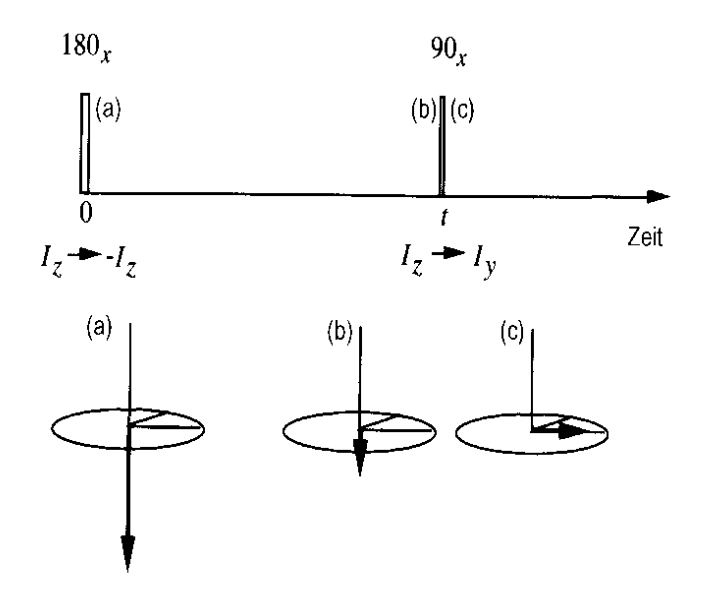
\includegraphics[width=0.4\textwidth]{Plots/inversionserholung.png}
	\caption{Oben die Pulsreihenfolge f\"{u}r eine Inversionserholung zur Messung der $T_1$-Zeit. Darunter ist die dazugeh\"{o}rige Magnetisierung veranschaulicht.}
	\label{inversion}
\end{SCfigure}
Nach den zwei eingeschalteten Pulsen zerf\"{a}llt die erzeugte Quer{\-}mag{\-}ne{\-}ti{\-}sie{\-}rung wieder und ein FID-Signal ist messbar.
Da die Amplitude dieses Signals proportiuonal zu der longitudinalen Magnetisierung ist, kann daraus dann die Relaxationszeit $T_1$ bestimmt werden.
Zus\"{a}tzlich dazu kann aus der ersten Blochgleichung die zeitabh\"{a}ngige longitudianle Magnetisierung ermittelt werden.
\begin{align*}
	M_z(t) = M_{eq} \left(1 - 2 exp\left( - \frac{t}{T_1} \right) \right)
\end{align*}
Um eine grobe Absch\"{a}tzung der longitudinalen Relaxationszeit vorzunehmen, kann folgende Gleichung verwendet werden:
\begin{align*}
	t_{\frac{1}{2}} = T_1 \cdot ln(2) \, \Rightarrow \, M_z(t) = 0
\end{align*}
Solch eine Absch\"{a}tzung ist wichtig, da sichergestellt werden soll, dass jede neue Messung wieder mit im Gleichgewichtszustand starten soll.
Um dies zu gew\"{a}hrleisten sollt zwischen zwei Messungen eine Wartezeit von $t \approx 4 \cdot T_1$ sein.
Dadruch wird auch das Sihnal-zu-Rauch-Verh\"{a}ltnis verbessert.

Neben der Inversionserholung gibt es noch die M\"{o}glichkeit mittels einer S\"{a}ttigungs{\-}erhol{\-}ung die $T_1$-Zeit du bestimmen.
Hierbei wird zun\"{a}chst die Magnetisierung duch zuf\"{a}llig hintereinander geschaltete Pulse zerst\"{o}rt.
Durch den Wideraufbau der L\"{a}ngmagnetisierung kann dann die $T_1$-Zeit bestimmt werden.

\paragraph{Spin-Spin-Relaxation}
\begin{wrapfigure}[12]{r}{0.35\textwidth}
	\centering
	\vspace{-10pt}
	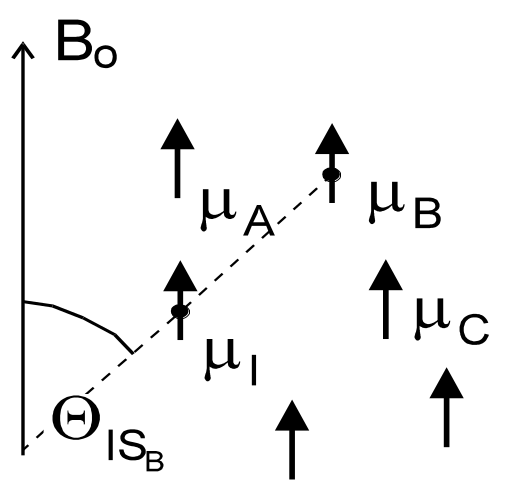
\includegraphics[width=0.3\textwidth]{Plots/spin_spin.png}
	\caption{Schematische Darstellung der Spin-Spin-Wechselwirkung.}
	\label{SpinSpin}
\end{wrapfigure}
Die zweite Relaxation be{\-}ruht auf der Spin-Spin-Wechselwirkung, welche auch als magnetische Wechselwirkung zwischen den Dipolen aufgefasst werden kann.
Und anders als bei der Spin-Gitter-Relaxation flie{\ss}t hierbei kein Energiefluss ins Gitter.
Durch die Wechselwirkung zwischen den Spins ist die St\"{a}rke der Zusatzfelder abh\"{a}ngig von dem Winkel, $\vartheta$, zwischen $B_0$ und $r$ (Abbildung (\ref{SpinSpin})).
Mathematisch ergeben sich die Zusatzfelder der Nachbarspins zu:
\begin{align*}
	B_z^{DD} &= \sum_s \hbar \gamma_s S \left( 3 cos^2 \left(\vartheta_{IS}\right) - 1 \right) \frac{1}{r_{IS}^3} \\
	\text{und} \, \, \, \, B_{x,y}^{DD} &= \sum_s \hbar \gamma_s S \left( \frac{3}{2} \cdot sin\left(2 \vartheta_{IS}\right) \right) \frac{1}{r_{IS}^3} 
\end{align*}

Im Vergleich zu $T_1$-Relaxationszeit ist die Spin-Spin-Relaxationszeit $T_2$ in Festk\"{o}rpern immer kleiner.
Nur in Fl\"{u}ssigkeiten sind beide Relaxationszeiten in dergleichen Gr\"{o}{\ss}enordnung.

\subsection{Hahn-Echo und Festk\"{o}rper-Echo}
1. Hahn-Echo
- f\"{u}r die Refokussierung von Wechselwirkungen, die linear in $\widehat{I}_z$ sind
- zum Beispiel: chemische Verschiebung, Dipol-Dipol-Wechselwirkung, Inhomogenit\"{a}ten von $B_{ext}$
-> mit $\widehat{H}_z = \omega \widehat{I}_z$
-> $90^{\circ}$-Puls und $180^{\circ}$-Puls
\begin{figure}[hbtp]
	\centering
	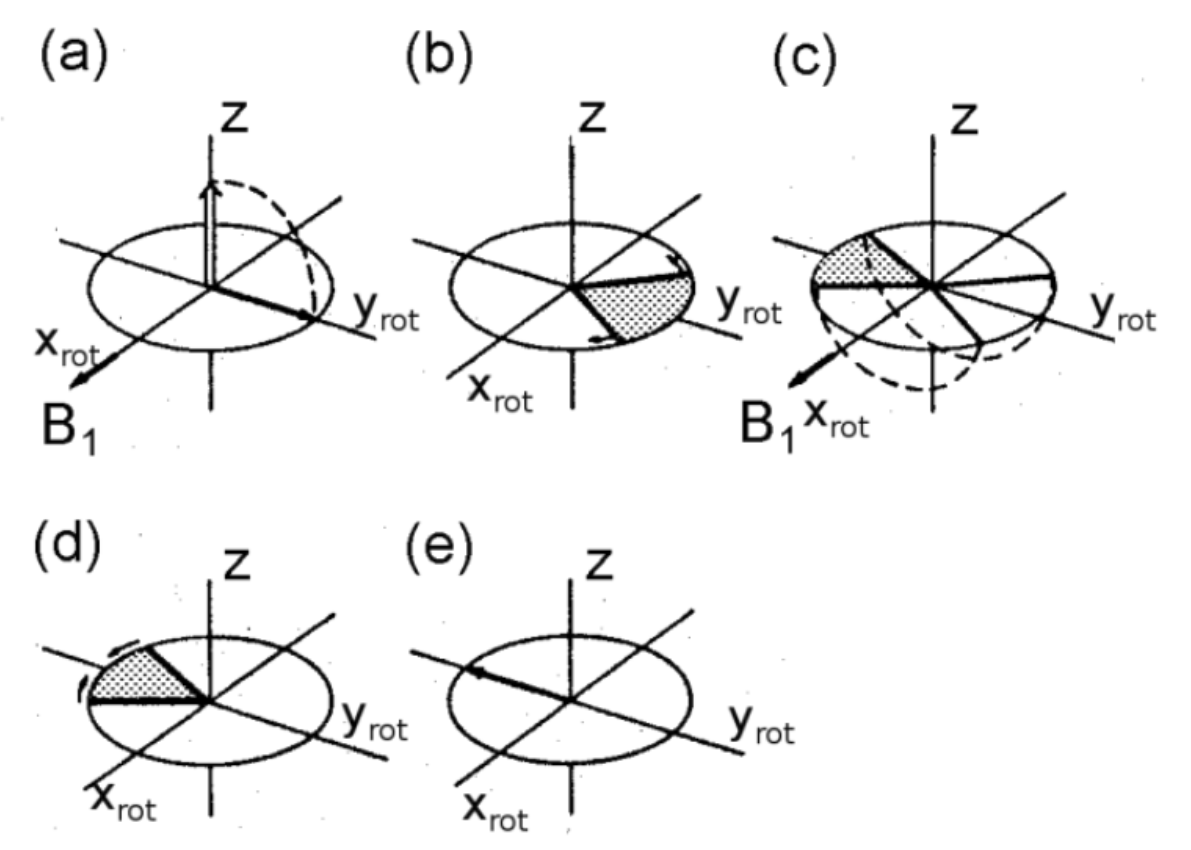
\includegraphics[width=0.5\textwidth]{Plots/hahnEcho.png}
	\caption{Hahn-Echo}
	\label{hahn}
\end{figure}


2. Festk\"{o}rper-Echo
- f\"{u}r die Refokussierung von Wechselwirkung die linear in homonuklearen Spinoperatoren 
-> $90^{\circ}$-Puls X und $90^{\circ}$-Puls, der um $\frac{\pi}{2}$ mit dem ersten Puls au{\ss}er Phase ist ($\pm Y$)
\begin{figure}
\centering
	\begin{subfigure}[b]{0.4\textwidth}
		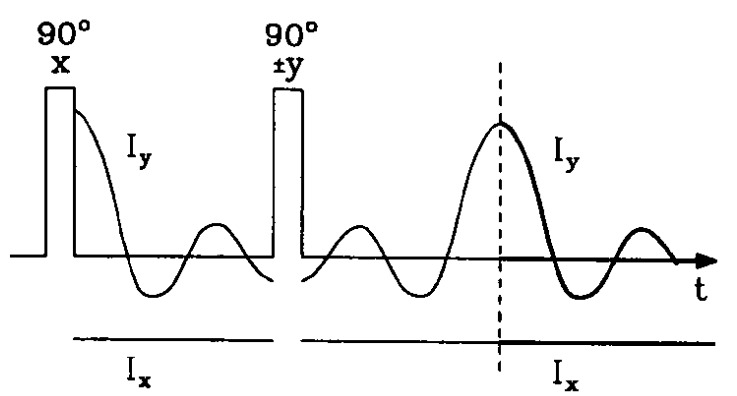
\includegraphics[width=\textwidth]{Plots/festkoerperecho.png}
		\caption{.}
		\label{.}
	\end{subfigure}
	~
	\begin{subfigure}[b]{0.4\textwidth}
		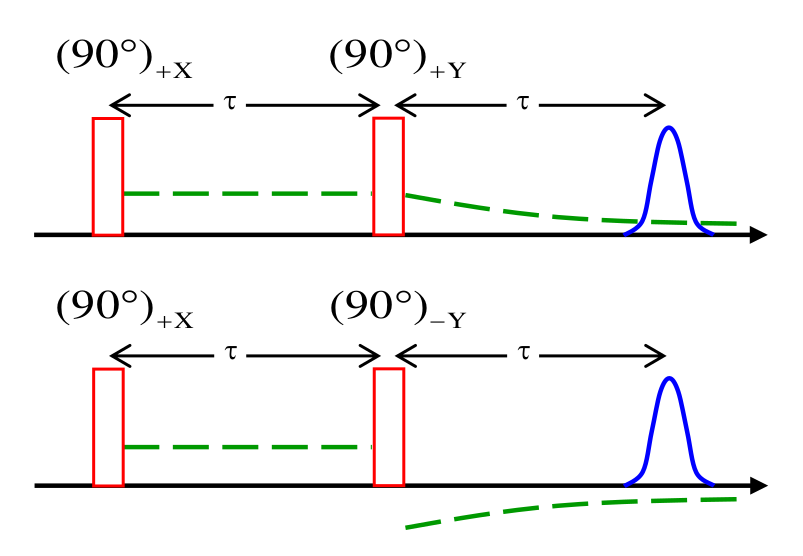
\includegraphics[width=\textwidth]{Plots/festkoerperecho2.png}
		\caption{.}
		\label{.}
	\end{subfigure}
\caption{Festk\"{o}rper-Echo}
\label{.}
\end{figure}


\subsection{Der $^2$H-Kernspin-Hamiltonoperator}
- aufspaltung
- Quadropolwechselwirkung
\begin{figure}[hbtp]
	\centering
	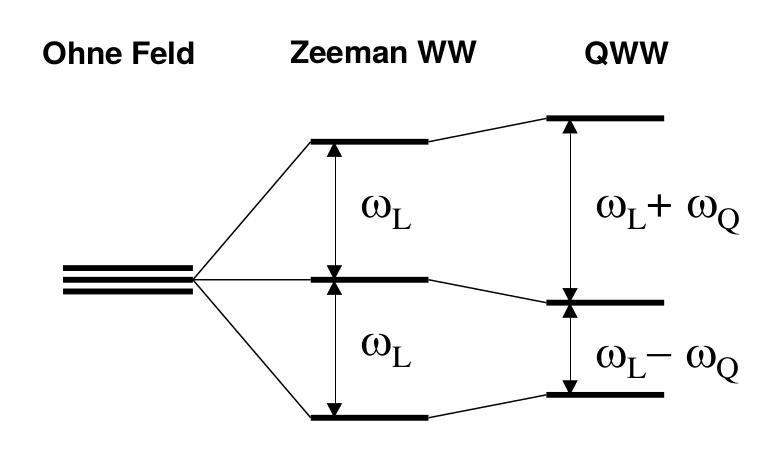
\includegraphics[width=0.4\textwidth]{Plots/aufspaltung.png}
	\caption{Aufspaltung}
	\label{}
\end{figure}



\subsection{Stimuliertes Echo}
-> Korrelationszeit
\begin{figure}
\centering
	\begin{subfigure}[b]{0.4\textwidth}
		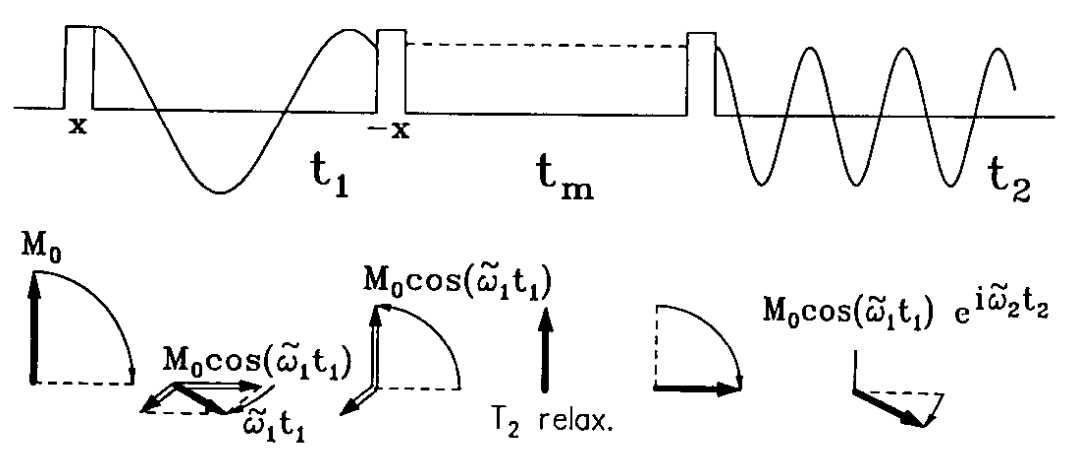
\includegraphics[width=\textwidth]{Plots/stimuliertesecho.png} 
		\caption{.}
		\label{.}
	\end{subfigure}
	~
	\begin{subfigure}[b]{0.4\textwidth}
		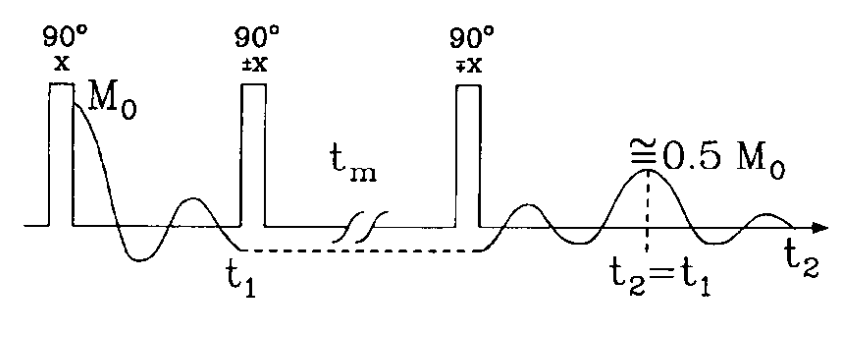
\includegraphics[width=\textwidth]{Plots/stimuliertesecho2.png}
		\caption{.}
		\label{.}
	\end{subfigure}
\caption{Festk\"{o}rper-Echo}
\label{.}
\end{figure}

\begin{figure}[hbtp]
	\centering
	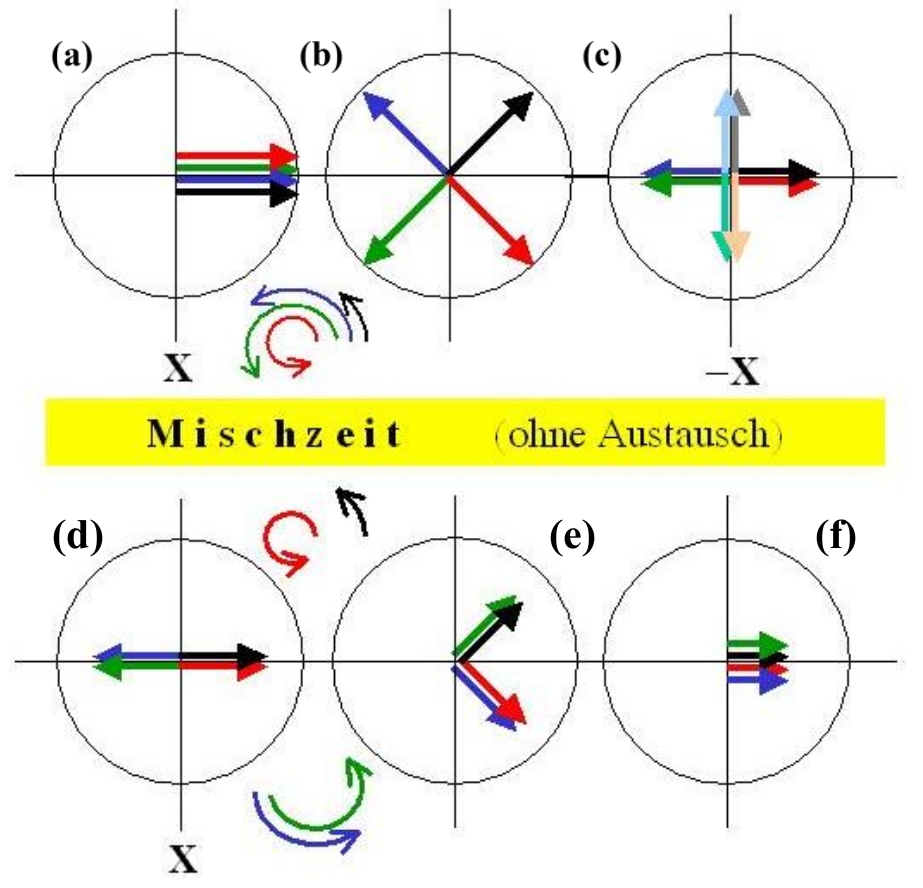
\includegraphics[width=0.5\textwidth]{Plots/mischzeit.png}
	\caption{.}
	\label{.}
\end{figure}
